
\newpage
\chapter{Stromkreis}

In der \fref{fig:circuit_battery} ist ein Stromkreis gezeigt.
Er besteht aus einer Spannungsquelle (Batterie), einem Verbraucher (Glühlampe)
und einem Hin- und einem Rückleiter (rotes und schwarzes Kabel).

Man kann einen Stromkreis auch als Schaltplan darstellen, siehe \fref{fig:circuit_schematic}.
Die Spannungsquelle ist durch ein Batteriesymbol und der Verbraucher durch ein
Lämpchensymbol dargestellt Verbunden sind sie durch die Kabel, welche
als durchgezogene Linien dargestellt werden.

\begin{figure}[h!]
\centering
    \begin{subfigure}[b]{0.46\textwidth}
    \centering
    \includegraphics[width=6cm]{_images/stromkreis_schaltplan}
    \caption{\label{fig:circuit_schematic}}
    \end{subfigure}
\quad
    \begin{subfigure}[b]{0.46\textwidth}
    \centering
    \includegraphics[width=5.5cm]{_images/stromkreis_batterie}
    \caption{\label{fig:circuit_battery}}
    \end{subfigure}

    \caption{Schaltplan und Aufbau eines Stromkreises}
\end{figure}

Eine Spannungsquelle (Batterie) erzeugt eine elektrische Spannung, die
die Elektronen in den Kabel in Bewegung setzen. Die Elektronen bewegen sich durch die
Kabel und durch die Verbraucher (Glühlampe). Die Verbraucher sind Geräte, die
elektrische Energie in andere Energieformen umwandeln, z.B. in Wärme,
Licht oder Bewegung.





\newpage
\experiment{Einfacher Stromkreis}

Baue das Experiment aus siehe \fref{fig:experiment_circuit} auf. Verwende eine Batterie, eine Glühbirne und einen Schalter.
Beachte, dass die Batterie so eingebaut wird, dass der Pluspol beim roten und der Minuspol
beim schwarzen Anschluss zu liegen kommt. Schliesse den Stromkreis und beobachte, was passiert.

\begin{figure}[h!]
    \centering
    \includegraphics[width=9cm]{_images/stromkreis.pdf}
    \caption{Stromkreis}
    \label{fig:experiment_circuit}
\end{figure}

Beantworte die folgende Fragen: Was passiert, wenn ...

\begin{enumerate}
    \item ein Kabel aus dem Stromkreis entfernt wird?
    \item die Batterie umgedreht wird?
    \item der Schalter und die Glühbirne vertauscht werden?
\end{enumerate}

% Raster für die Antworten
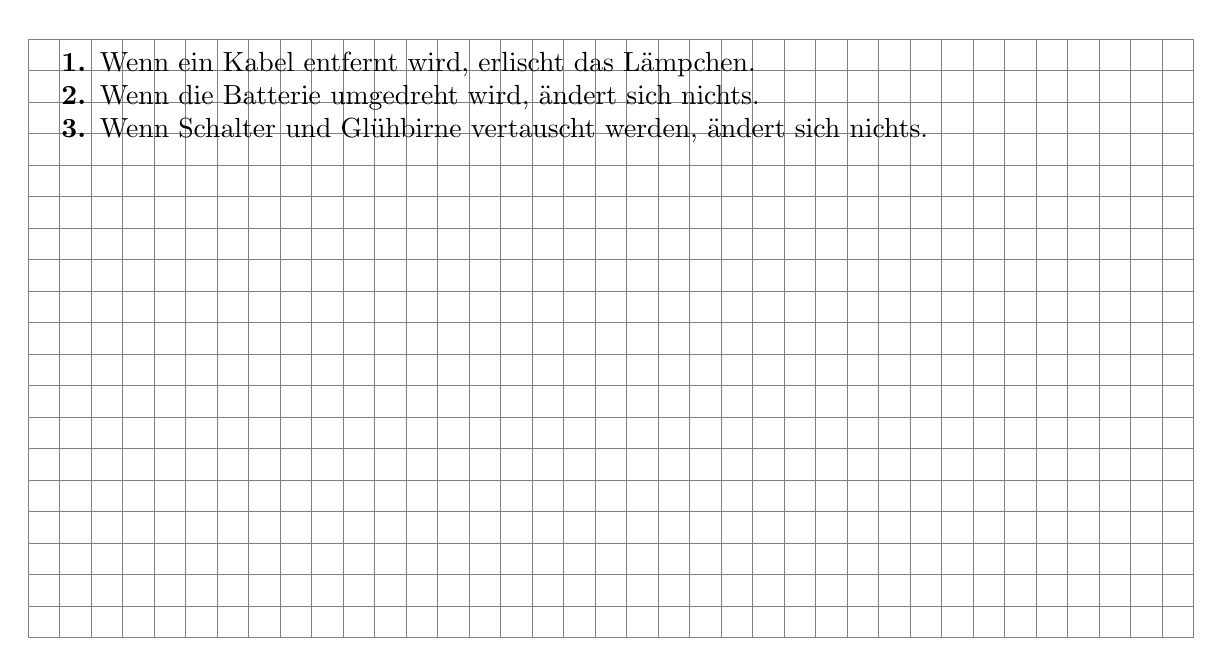
\begin{tikzpicture}
    \draw[step=4mm,gray,very thin] (0,0) grid (14.8,-7.6);

    \answer{
        \draw (0.3,0.14) node[anchor=north west,align=left,text width=13cm] {%
    		\marker%

            \textbf{1.} Wenn ein Kabel entfernt wird, erlischt das Lämpchen.\\
            \textbf{2.} Wenn die Batterie umgedreht wird, ändert sich nichts.\\
            \textbf{3.} Wenn Schalter und Glühbirne vertauscht werden, ändert sich nichts.\\
        };
    }
\end{tikzpicture}


\newpage
\section{Das Wassermodell eines Stromkreises}
Es gibt eine Analogie zwischen einem Stromkreis und einem Wasserkreislauf.
Das Wasser wird mit einem Schöpflöffel (Batterie) von dem Behälter
mit tieferem Wasserstand (Minuspol) in den Behälter mit höherem Wasserstand
(Pluspol) geschöpft. Durch das Gefälle fliesst das Wasser durch die Rohre
(Kabel) und treibt das Wasserrad (Glühlampe) an, siehe \fref{fig:watermodel}.
Der Schalter entspricht einem Ventil, das den Wasserfluss unterbricht.


\begin{figure}[h!]
    \centering
    \includegraphics[width=11cm]{_images/wassermodell_stromkreis.pdf}
    \caption{Analogie: Wassermodell eines Stromkreises}
    \label{fig:watermodel}
\end{figure}

Lässt man das Wasser fliessen, ohne Wasser nachzuschöpfen, gleichen sich
die Wasserstände in den Behältern langsam an und das Wasserrad dreht langsamer.
Nach einer gewissen Zeit werden sich die Wasserstände in den Behältern gleich
sein und es fliesst kein Wasser mehr. Die Batterie ist nun leer und muss wieder
mit dem Schöpflöffel aufgefüllt werden.






\newpage
\exercise{Die Wirkungen vom elektrischen Strom}

Strom kann unter anderem Licht, Wärme, Schall, Bewegung und Magnetismus erzeugen.
Verbinde die Wirkungen mit den Geräten, die sie erzeugen.

\begin{tikzpicture}
    \draw[step=4mm,lightgray,very thin] (0,0) grid (14.8,-20);



    \node[fill=white,draw,very thick,inner sep=0.5cm,rounded corners, rotate=-2] (motion) at (3,-2) {\marker%
        Bewegung
    };

    \node[fill=white,draw,very thick,inner sep=0.5cm,rounded corners, rotate=2] (sound) at (3,-6) {\marker%
        Schall
    };

    \node[fill=white,draw,very thick,inner sep=0.5cm,rounded corners, rotate=3] (heat) at (3,-10) {\marker%
        Wärme
    };

    \node[fill=white,draw,very thick,inner sep=0.5cm,rounded corners, rotate=2] (magnet) at (3,-14) {\marker%
        Magnetismus
    };

    \node[fill=white,draw,very thick,inner sep=0.5cm,rounded corners, rotate=-1] (light) at (3,-18) {\marker%
        Licht
    };


    \node[rotate=3] (speaker) at (11,-2)
        {\includegraphics[width=5cm]{_images/wirkung_lautsprecher}}; % Eric Nopanen / Unsplash

    \node[rotate=1] (lamp) at (12,-6)
            {\includegraphics[width=5cm]{_images/wirkung_lampe}}; % Daniel Herron / Unsplash

    \node[rotate=-2] (fan) at (11,-10)
            {\includegraphics[width=5cm]{_images/wirkung_ventilator}}; % Daniil Onischenko / Unsplash

    \node[rotate=-3] (toaster) at (12,-14)
            {\includegraphics[width=5cm]{_images/wirkung_toaster}}; % CC0 / pxhere.com

    \node[rotate=2] (crane) at (11,-18)
            {\includegraphics[width=5cm]{_images/wirkung_magnet}}; % hvrmagnet.com


    \answer{
        \draw [very thick, dashed]
            (heat.east) .. controls ++(0:2) and ++(180: 2) .. (speaker.west)
            (heat.east) .. controls ++(0:2) and ++(180: 2) .. (lamp.west)
            (heat.east) .. controls ++(0:2) and ++(180: 2) .. (fan.west)
            (heat.east) .. controls ++(0:2) and ++(180: 2) .. (crane.west);

        \draw [very thick]
            (motion.east) .. controls ++(0:2) and ++(180: 2) .. (fan.west)
            (sound.east) .. controls ++(0:2) and ++(180: 2) .. (speaker.west)
            (heat.east) .. controls ++(0:2) and ++(180: 2) .. (toaster.west)
            (light.east) .. controls ++(0:2) and ++(180: 2) .. (lamp.west)
            (magnet.east) .. controls ++(0:2) and ++(180: 2) .. (crane.west);

    }


\end{tikzpicture}



\newpage
\section{Serien- und Parallelschaltung}

Bei der <<Serienschaltung>> oder <<Reihenschaltung>> sind die Verbraucher
wie in einer Kette hintereinander angeordnet. Der gleiche elektrische Strom fliesst
durch alle Verbraucher nacheinander. Es gibt keine Verzweigungen und somit
nur einen Stromkreis. Ein Beispiel für ist eine Lichterkette
der Weihnachtsbeleuchtung, siehe \fref{fig:christmaslights}.

\begin{figure}[h!]
\centering
    \begin{subfigure}[b]{0.46\textwidth}
    \centering
    \includegraphics[width=6cm]{_images/weihnachtsbeleuchtung}
    \caption{\label{fig:christmaslights}}
    \end{subfigure}
    \quad
    \begin{subfigure}[b]{0.46\textwidth}
    \centering
    \includegraphics[width=5.5cm]{_images/serienschaltung_schaltplan}
    \caption{\label{fig:series_schematic}}
    \end{subfigure}

    \caption{Weihnachtsbeleuchtung und Schaltplan}
\end{figure}



Bei der <<Parallelschaltung>> sind die Verbraucher alle direkt an
die Spannungsquelle angeschlossen, siehe \fref{fig:parallel_schematic}.
Es gibt mehrere Knotenpunkte, an bei denen der Strom sich verzweigt.
Somit hat jeder Verbraucher seinen eigenen Stromkreis.
Ein Beispiel ist eine Steckdose, bei der mehrere Geräte angeschlossen werden
können, wie in \fref{fig:powerstrip} gezeigt.

\begin{figure}[h!]
\centering
    \begin{subfigure}[b]{0.46\textwidth}
    \centering
    \includegraphics[width=6cm]{_images/steckdosenleiste}
    \caption{\label{fig:powerstrip}}
    \end{subfigure}
\quad
    \begin{subfigure}[b]{0.46\textwidth}
    \centering
    \includegraphics[width=5.5cm]{_images/parallelschaltung_schaltplan}
    \caption{\label{fig:parallel_schematic}}
    \end{subfigure}

    \caption{Weihnachtsbeleuchtung und Steckdosenleiste}
\end{figure}



\newpage
\experiment{Serienschaltung}

Baue das Experiment aus siehe \fref{fig:experiment_lamps_series} auf. Die
Lampen und die Batteriensind nacheinander, d.h. in Serie geschaltet.

\begin{figure}[h!]
    \centering
    \includegraphics[width=9cm]{_images/lampen_serie.pdf}
    \caption{Lampen in einer Serienschaltung}
    \label{fig:experiment_lamps_series}
\end{figure}

Beantworte die folgenden Fragen:

\begin{enumerate}
    \item Was passiert, wenn ein Lämpchen <<kaputt>> geht. Drehe es dazu aus der Fassung.
    \item Was passiert, wenn du nur eine anstatt zwei Batterien verwendest?
    \item Vervollständige den Schaltplan.
\end{enumerate}

% Raster für die Antworten
\begin{tikzpicture}
    \draw[step=4mm,gray,very thin] (0,0) grid (14.8,-8.4);

    \noanswer{
        \node  at (7,-6)
            {\includegraphics[width=8cm]{_images/lampen_serie_schaltplan.pdf}};
    }
    \answer{
        \node  at (7,-6)
            {\includegraphics[width=8cm]{_images/lampen_serie_schaltplan_loesung.pdf}};
    }
    \answer{
        \draw (0.3,0.14) node[anchor=north west,align=left,text width=13cm] {%
            \marker%

            \textbf{1.} Wenn ein Lämpchen kaputt geht, erlischt das andere auch.\\
            \textbf{2.} Wenn man nur eine Batterie verwendet, brennen die Lämpchen nur noch ganz schwach. \\
        };
    }
\end{tikzpicture}





\newpage
\experiment{Parallelschaltung}

Baue das Experiment aus siehe \fref{fig:experiment_lamps_parallel} auf. Die
Lampen und die Batteriensind nebeneinander, d.h. in Parallel geschaltet.

\begin{figure}[h!]
    \centering
    \includegraphics[width=9cm]{_images/lampen_parallel.pdf}
    \caption{Lampen in einer Parallelschaltung}
    \label{fig:experiment_lamps_parallel}
\end{figure}

Beantworte die folgenden Fragen:

\begin{enumerate}
    \item Wie hell leuchten die Lampen im Vergleich zu einer Serienschaltung?
    \item Was passiert, wenn ein Lämpchen kaputt geht. Drehe es dazu aus der Fassung.
    \item Vervollständige den Schaltplan.
\end{enumerate}

% Raster für die Antworten
\begin{tikzpicture}
    \draw[step=4mm,gray,very thin] (0,0) grid (14.8,-8.4);

    \noanswer{
        \node  at (7,-6)
            {\includegraphics[width=8cm]{_images/lampen_parallel_schaltplan}};
    }
    \answer{
        \node  at (7,-6)
            {\includegraphics[width=8cm]{_images/lampen_parallel_schaltplan_loesung}};
    }
    \answer{
        \draw (0.3,0.14) node[anchor=north west,align=left,text width=13cm] {%
    		\marker%

            \textbf{1.} Die Lämpchen leuchten heller als in bei der Serienschaltung. \\
            \textbf{2.} Wenn ein Lämpchen kaputt geht, leuchtet das andere weiterhin.\\
        };
    }
\end{tikzpicture}


\exercise{In Serie oder Parallel?}

Bestimme bei den gezeigten Schaltplänen, ob die Lampen in Serie oder Parallel geschaltet sind.

\begin{tikzpicture}
    \draw[step=4mm,lightgray,very thin] (0,0) grid (14.8,-8);

    \node at (0.6,-0.5) {a)};
    \node at (3.5,-3)
            {\includegraphics[width=7cm]{_images/serie_parallel_aufgabe_1}};

    \node at (8.6,-0.5) {b)};
    \node at (11.5,-3)
            {\includegraphics[width=7cm]{_images/serie_parallel_aufgabe_2}};


    \answer{
        \draw (0.3,-5.14) node[anchor=north west,align=left,text width=13cm] {%
    		\marker%

            \textbf{a)} L$_{\text{2}}$ und L$_{\text{3}}$ sind zueinander parallel. L$_{\text{1}}$ ist in Serie zu L$_{\text{2}}$ und L$_{\text{3}}$. \\

            \textbf{b)} Gleich wie Aufgabe a)\\
        };
    }


\end{tikzpicture}






\section{Kurzschluss}

Manchmal kann es zu einem Kurzschluss kommen, wenn man aus Versehen eine direkte Verbindung
zwischen den Batteriepolen macht. In diesem Fall kann
es zu einem Überstrom kommen, welcher die Kabel oder die Batterie zerstört.

Wenn etwa ein Haushaltsgerät kaputtgeht, kann es auch zu einem Kurzschluss kommen.
Oft sind es alte Steckerleisten, welche nicht mehr richtigen Kontakt haben. Sie können
sich aufheizen und schmelzen, siehe \fref{fig:short_circuit}.

\begin{figure}[h!]
    \centering
    \includegraphics[width=9cm]{_images/kurzschluss}
    \caption{Kurzschluss bei einer Steckerleiste (Bild erstellt mit DALL·E, OpenAI)}
    \label{fig:short_circuit}
\end{figure}

\begin{redbox}
Kurzschlüsse müssen vermieden werden. Es ist wichtig, nur intakte Bauteile zu verwenden und
nur die gezeigten Schaltungen aufzubauen und vor dem Einschalten zu überprüfen.
\end{redbox}



\newpage
\experiment{Kurzschluss}


Baue das Experiment aus siehe \fref{fig:experiment_short_circuit} auf. Der Kurzschluss über
der rechten Lampe ist nicht gefährlich. Der gesamte Strom geht über das Kabel.
Eine Gefahr besteht, wenn man die Batteriepole direkt kurzschliesst.

\begin{figure}[h!]
    \centering
    \includegraphics[width=9cm]{_images/kurzschluss_aufbau.pdf}
    \caption{Aufbau eines Kurzschlusses}
    \label{fig:experiment_short_circuit}
\end{figure}

Schliesse den Schalter und notiere deine Beobachtungen. Beantworte die folgenden Fragen:

\begin{enumerate}
    \item Was passiert mit der rechten Lampe?
    \item Was passiert, wenn du nur die linke Lampe kurzschliesst?
    \item Was bedeutet das für den elektrischen Strom?
\end{enumerate}

% Raster für die Antworten
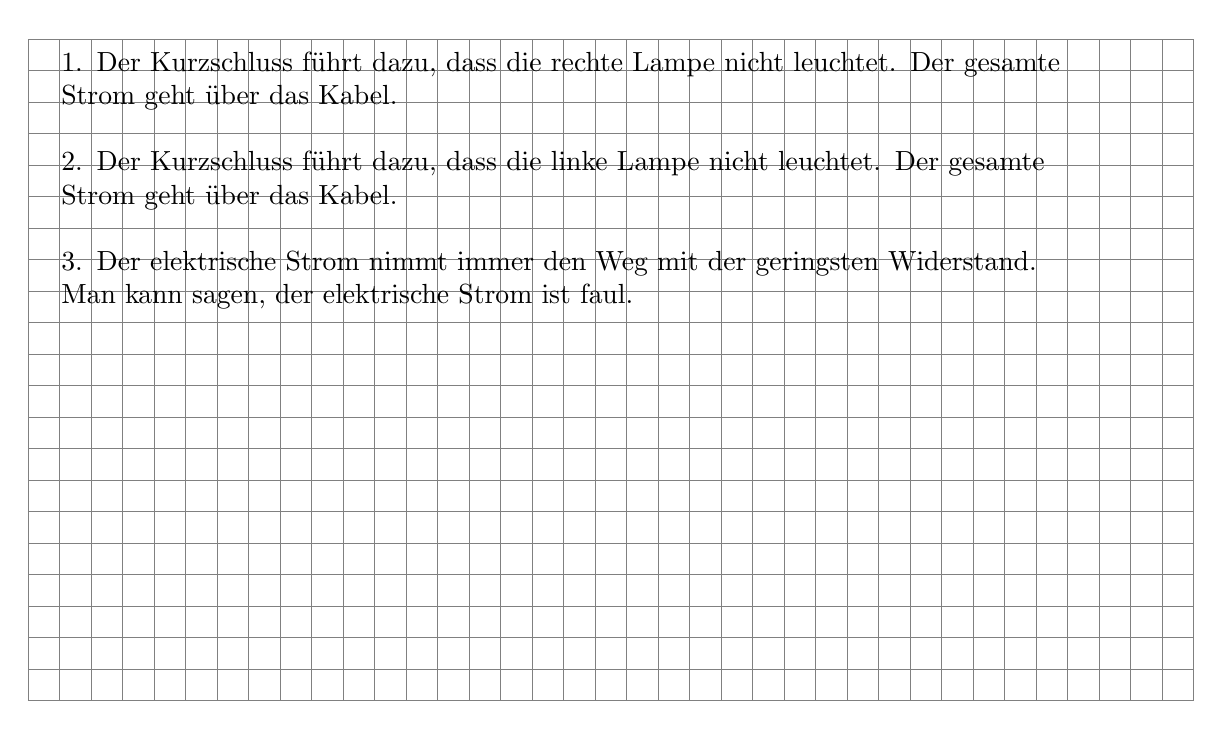
\begin{tikzpicture}
    \draw[step=4mm,gray,very thin] (0,0) grid (14.8,-8.4);

    \answer{
        \draw (0.3,0.14) node[anchor=north west,align=left,text width=13cm] {%
    		\marker%

            1. Der Kurzschluss führt dazu, dass die rechte Lampe nicht leuchtet. Der gesamte Strom
            geht über das Kabel. \\
            \ \\
            2. Der Kurzschluss führt dazu, dass die linke Lampe nicht leuchtet. Der gesamte Strom
            geht über das Kabel. \\
            \ \\
            3. Der elektrische Strom nimmt immer den Weg mit der geringsten Widerstand. Man kann
            sagen, der elektrische Strom ist faul.
        };
    }
\end{tikzpicture}
